\documentclass[a4paper]{jpconf}
% \bibliographystyle{iopart-num}
\usepackage{amsmath}
\usepackage{citesort}
\usepackage{subfigure}
\usepackage{graphicx}
\graphicspath{{fig/}}
\usepackage{ifpdf}
\ifpdf\usepackage{epstopdf}\fi
\usepackage[export]{adjustbox}

%----------------------------------------------------- 
%\usepackage{soul,ulem,color,xspace,bm}
% Suggest to remove
%\newcommand{\asrm}[1]{{\color{magenta}\sout{#1}}}
% Suggest to insert
%\newcommand{\as}[1]{\color{cyan}#1\xspace\color{black}}
% Suggest to replace
%\newcommand{\asrp}[2]{\asrm{#1} \as{#2}}
% Comment
%\newcommand{\ascm}[1]{{\color{green}\;AS: #1}}
%------------------------------------------------------

\def\apj{ApJ}
\def\mnras{MNRAS}
\def\nat{Nat}
\def\prd{Phys. Rev. D}
\def\araa{ARA\&A}                % "Ann. Rev. Astron. Astrophys."
\def\aap{A\&A}                   % "Astron. Astrophys."
\def\aaps{A\&AS}                 % "Astron. Astrophys. Suppl. Ser."
\def\aj{AJ}                      % "Astron. J."
\def\apjs{ApJS}                  % "Astrophys. J. Suppl. Ser."
\def\pasp{PASP}                  % "Publ. Astron. Soc. Pac."
\def\apjl{ApJ}                   % letter at ApJ
\def\pasj{PASJ}
\def\apss{Astroph. Space Sci.}
\def\aplett{Astroph. Lett}
\def\ssr{Space Sci. Rev.}
\def\aapr{Astron. Astroph. Reviews}
\def\physrep{Phys. Reports}
\def\memsai{Mem. Societa Astronom. Italiana}
\def\jgr{JGR}
\def\jcap{Journal of Cosmology and Astroparticle Physics}

\usepackage{xspace}
\usepackage[dvipsnames]{xcolor}
\usepackage[normalem]{ulem}
% Suggest to remove
\newcommand{\asrm}[1]{{\color{OrangeRed}\sout{#1}}}
% Suggest to insert
\newcommand{\as}[1]{\color{RoyalBlue}#1\xspace\color{black}}
% Suggest to replace
\newcommand{\asrp}[2]{\asrm{#1} \as{#2}}
% Comment
\newcommand{\ascm}[1]{{\color{ForestGreen}#1}}

\begin{document}
	\title{PIC simulation of instabilities in relativistic supernovae shocks}
	
	\author{V I Romansky$^{1}$, A M Bykov$^{1,2}$ and S M Osipov$^{1}$}
	
	\address{$^1$ Ioffe Institute, 26 Politekhnicheskaya st., St. Petersburg 194021, Russia}
	\address{$^2$ Peter the Great St. Petersburg Polytechnic University, 29 Politekhnicheskaya st., St. Petersburg 195251, Russia}
	
	\ead{romanskyvadim@gmail.com}
	
	\begin{abstract}
                 Radio observations revealed a presence of relativistic supernovae a class of objects intermediate between regular supernovae and gamma-ray bursts. The typical Lorentz-factors of plasma flows in relativistic radio-bright supernovae were estimated to be about 1.5. Mildly relativistic shocks in electron-ion plasmas are known to efficiently accelerate radio-emitting electrons if the shock is subluminous. The inclination angle of the subluminous shock to the ambient magnetic field should be below a critical angle which depends on the Mach number and the plasma magnetization parameter.  In this paper we present particle-in-cell modeling of electron acceleration by a subluminal mildly-relativistic collisionless shock. It is shown that  a development of the ion scale Bell-type instability in electron-ion relativistic shock may have a strong influence on the electron injection and acceleration. In time period of about $1500 \omega_{pi}^{-1}$  ($\omega_{pi}$ is the ion plasma frequency) after the shock initialization the  magnetic field fluctuations  generated by Bell's instability may significantly suppresses the electrons spectrum even in a sub-luminous shock. This effect is important to account for modeling of synchrothron spectra from relativistic supernovae.
	\end{abstract}
	
	\section{Introduction}
	Relativistic shocks are widely discussed phenomena in modern astrophysics. They can be generated in the supernovae \cite{2010Natur.463..513S,2007ApJ...667..351W}, the accreting supermassive black holes \cite{1984RvMP...56..255B}, the stellar masses black holes \cite{2019MmSAI..90...57M,1999PhR...314..575P,2014LNP...876.....R} and pulsar wind nebulae \cite{2019MNRAS.488.5690O,2017SSRv..207..235B,2017JPlPh..83e6301K,2019ApJ...876L...8B}. Relativistic shocks in astrophysical objects are sources of cosmic rays \cite{2012SSRv..173..309B,2015SSRv..191..519S,2017SSRv..207..319P} and can accelerate particles to ultra-high energies \cite{2009JCAP...11..009L}.
	
	The presence of high energy non-thermal particles leads to development of various magneto-hydrodynamic instabilities. Bell instability \cite{Bell04} can be the most significant due to it's large growth rate. Instabilities modify the flow and has strong influence on process of particle acceleration. We present below results of particle-in-cell modeling of relativistic shock and show that growth of magnetic field due to instabilities decreases efficiency of electron acceleration on shock front.
	
	
	\section{Numerical setup}
	In this work we use particle-in-cell code Smilei \cite{Smilei18} for modeling trans-relativistic collisionless shocks. We initialize two-dimensional space domain, with electron-proton plasma flowing into simulation box through the right boundary and reflecting wall on the left boundary. In the transversal direction boundary conditions are periodic.
	
	The simulation parameters are : the initial flow Lorentz factor $\Gamma = 1.5$, the flow magnetization $\sigma = \frac{B^2}{4\pi\Gamma (n_p m_p + n_e m_e) c^2} = 0.004$. The dimensionless thermal energy $\Delta \gamma = \frac{k T}{m_p c^2}$ is equal to $10^{-4}$ and the electron mass is increased up to $m_e = \frac{m_p}{100}$. The size of the simulation box along the $x$ axis is $L_x = 30000\frac{c}{\omega_p}$ and in the transverse direction $L_y = 200\frac{c}{\omega_p}$, where $\omega_p = \sqrt{\frac{4\pi q^2 n}{\Gamma m_e}}$ is the plasma frequency. These scales correspond to $150000$ and $1000$ grid points in $x$ and $y$ directions, respectively. 
	
	Inclination angle of magnetic field due to shock velocity varies in different setups from $\theta = 20$ degrees to $\theta = 40$. This values are chosen to contain critical angle, which is defined by the equation $c\cdot \cos(\theta_{crit})=v_{shock}$, where all values are measured in the upstream rest frame, and is equal approximately $30$ degrees. If inclination angle is larger then critical value, shock becomes superluminal - particle can not escape from it to upstream, even moving along the field lines with speed of light \cite{Pelletier2017,Sironi2011}. The maximum efficiency of particle acceleration is near the critical angle, less below it \cite{Romansky18}. Magnetic field is lying in the simulation plane.
	
	
	\section{Results}
	
	Profiles of transversal magnetic field, obtained from numerical simulation, show significant field amplification in precursor of shock wave, see figure \ref{field}. It is result of development of instabilities in plasma, particularly Bell's instability \cite{Bell04}, which growth rate is larger then growth rate of other instabilities.
	
	\begin{figure}[h!]
		\centering
		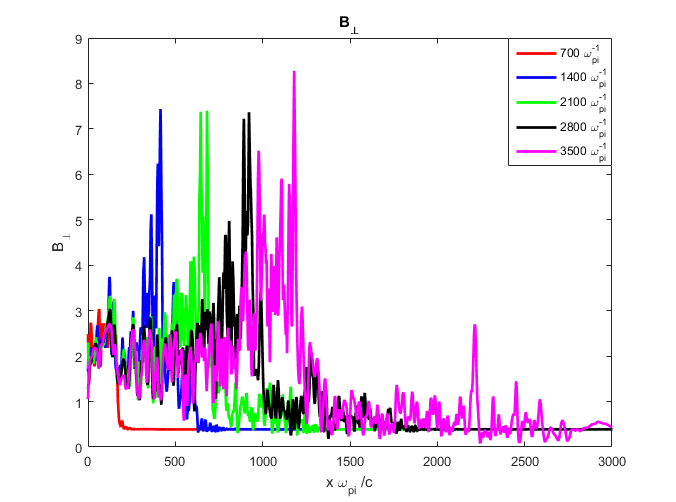
\includegraphics[width=0.8\textwidth]{fig/Bnorm.png} 
		\caption{Temporal evolution of the transversal magnetic field.}
		\label{field}
	\end{figure}
	
	It is known, that development of Bell's instability can suppress electrons acceleration \cite{Crumley2019}. We study this phenomena with different inclination angles of magnetic field. Spectrum of electrons is shown in figure \ref{spectrume}. One can see, that electrons distribution function at high energies $(\gamma > 300)$ is maximal at times about 1400 inverse protons plasma frequencies and at the longer times spectrum decreases. It may by explained as consequence of magnetic field amplification. Instabilities increase the transverse magnetic field and also the angle between field and shock velocity. As a result shock becomes quasi-perpendicular and can not effectively accelerate particles \cite{Sironi2011,Romansky18}. On the other hand, protons distribution function constantly increases in time, as shown in figure \ref{spectrump}. We assume, that oscillating transverse field has the strongest influence on the smallest scales, and suppresses the electrons injection into acceleration process.
	
	
	\begin{figure}[h!]
		\centering
		\begin{minipage}{0.49\textwidth}
			\centering
			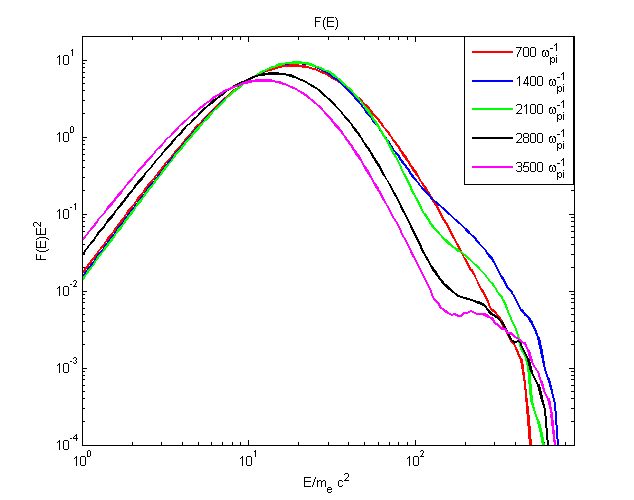
\includegraphics[width=0.95\textwidth]{fig/spectrum20.png} 
		\end{minipage}\hfill
		\begin{minipage}{0.49\textwidth}
			\centering
			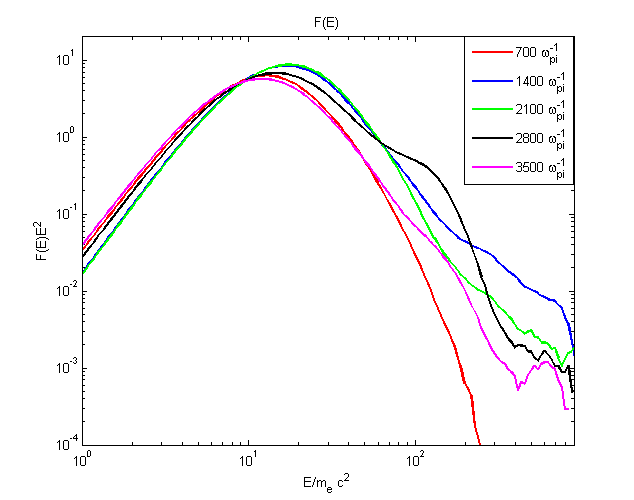
\includegraphics[width=0.95\textwidth]{fig/spectrum30.png} 
		\end{minipage}
		\begin{minipage}{0.49\textwidth}
			\centering
			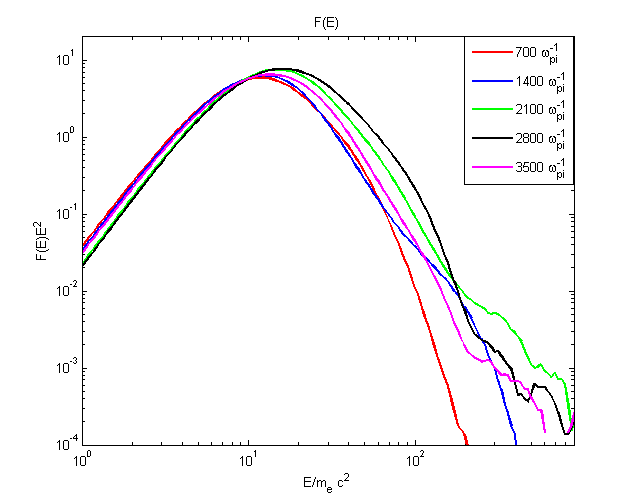
\includegraphics[width=0.95\textwidth]{fig/spectrum33.png} 
		\end{minipage}
		\begin{minipage}{0.49\textwidth}
			\centering
			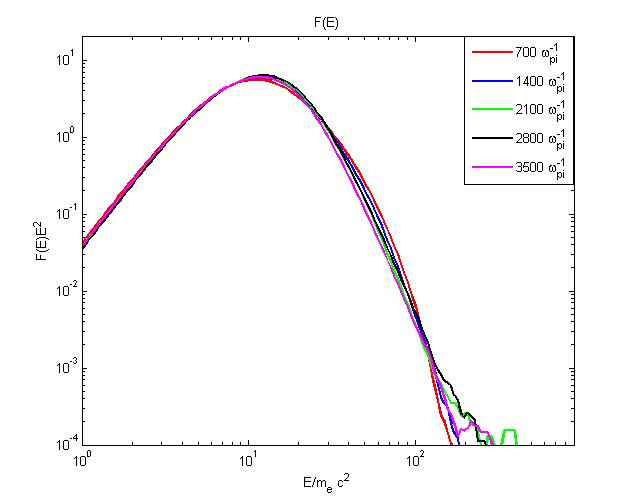
\includegraphics[width=0.95\textwidth]{fig/spectrum40.png} 
		\end{minipage}
		\caption{Temporal evolution of electrons spectrum in shocks with different inclination angles. Top row: left $\theta = 20^\circ$, right $\theta = 25^\circ$, bottom row: left $\theta = 33^\circ$, right $\theta = 40^\circ$}
		\label{spectrume}
	\end{figure}

\begin{figure}[h!]
	\centering
	\begin{minipage}{0.49\textwidth}
		\centering
		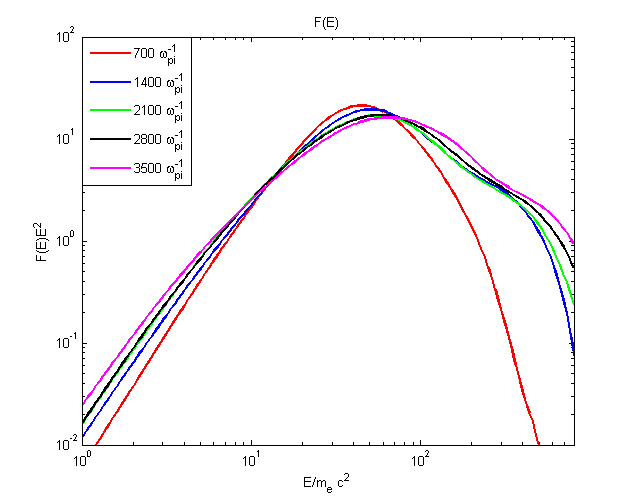
\includegraphics[width=0.95\textwidth]{fig/spectrump20.png} 
	\end{minipage}\hfill
	\begin{minipage}{0.49\textwidth}
		\centering
		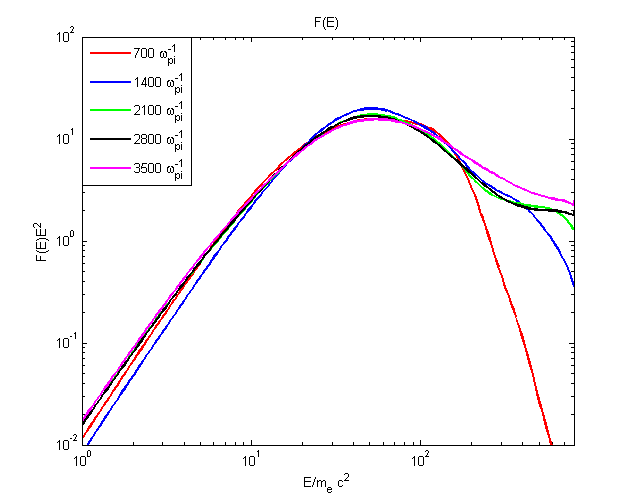
\includegraphics[width=0.95\textwidth]{fig/spectrump30.png} 
	\end{minipage}
	\begin{minipage}{0.49\textwidth}
		\centering
		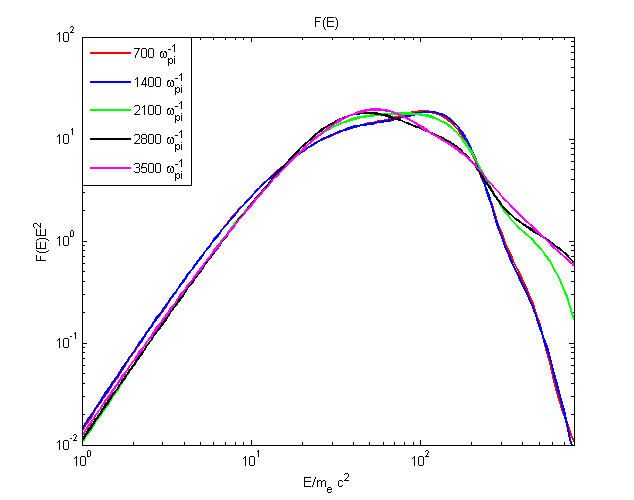
\includegraphics[width=0.95\textwidth]{fig/spectrump33.png} 
	\end{minipage}
	\begin{minipage}{0.49\textwidth}
		\centering
		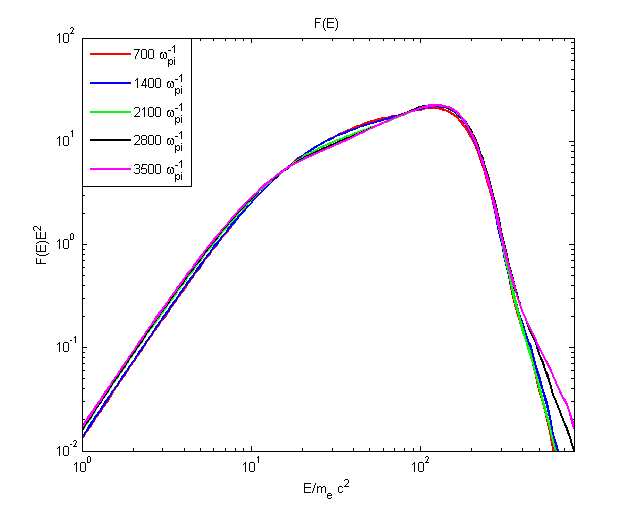
\includegraphics[width=0.95\textwidth]{fig/spectrump40.png} 
	\end{minipage}
	\caption{Temporal evolution of protons spectrum in shocks with different inclination angles. Top row: left $\theta = 20^\circ$, right $\theta = 25^\circ$, bottom row: left $\theta = 33^\circ$, right $\theta = 40^\circ$}
	\label{spectrump}
\end{figure}
	

	
	\section{Conclusions}
	
	Details of electrons acceleration are important for correct interpretations of observations synchrothron radiation from astrophysical sources. Particle-in-cell simulation has been used to demonstrate magnetic instabilities influence on electrons acceleration in relativistic electron-ion shock. It is shown, that amplification of magnetic field suppresses formation of electrons spectrum at high energies.This effect should be taken into account while deriving parameters of source of radiation via analysis of synchrothron spectrum. Further PIC simulations with a wider spatial and energetical ranges will allow to study the effect more precisely.
	
	
	\ack
	V I Romansky and A M Bykov acknowledge a support from RSF grant 16-12-10225.
	Results of the work were obtained using computational resources of Peter the Great Saint-Petersburg Polytechnic University Supercomputing Center (http://scc.spbstu.ru)
	
	\section*{References}
	% \bibliographystyle{apalike}
	\bibliographystyle{iopart-num}

	\bibliography{bibliogr}
\end{document}